\documentclass{article}
\usepackage{amsmath}
\usepackage{amssymb}
\usepackage{graphicx}
\usepackage{hyperref}
\usepackage[version=4]{mhchem}

\title{Problem 11}
\date{}

\begin{document}
\maketitle

\section*{Problem}
\(A B C D\) is a convex quadrilateral. Diagonlas \(A C=B D . A C\) and \(B D\) meet at \(O, E, F\) are midpoints of \(A B, C D\), respectively. \(E F\) meets \(B D\) at \(G\) and \(A C\) at \(H\). Show that \(O G=O H\).\\
\centering
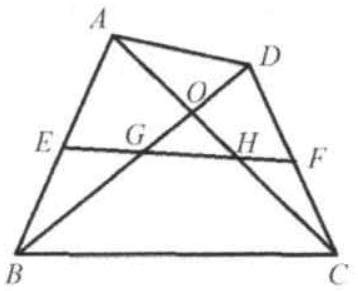
\includegraphics[width=\textwidth]{images/046.jpg}

\section*{Solution}
Take m , the midpoint of \(B C\).


Connect \(E M\) and \(F M\).\\
\(E M\) is the midline of \(\triangle B A C . E M / / A C\) and \(E M=\frac{1}{2} A C\)\\
\(F M\) is the midline of \(\triangle C B D . F M / / B D\) and \(F M=\frac{1}{2} B D\).\\
\centering
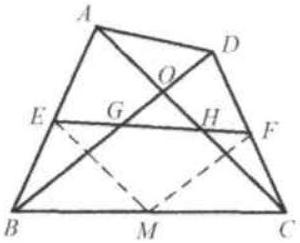
\includegraphics[width=\textwidth]{images/052.jpg}

Since \(A C=B D, E M=F M\). So \(\angle M E F=\angle M F E\).\\
Since \(E M / / A C, \angle M E F=\angle O H G\).\\
Since \(F M / / B D, \angle M F E=\angle O G H\).\\
Thus \(\angle O H G=\angle O G H\), and \(O G=O H\).

\section*{Chapter 3 Draw the Auxiliary lines with Angle Bisectors}
Angle Bisector
An angle bisector of a triangle is a segment or ray that bisects an angle and extends to the opposite side. As shown in the figure, \(A D\) is the angle bisector of \(\angle A\).\\
\(\angle 1=\angle 2\).

Theorem 3.1. The Angle Bisector Theorem
\begin{center}
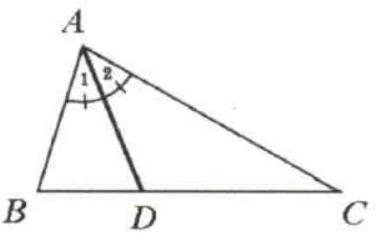
\includegraphics[width=\textwidth]{images/053.jpg}
\end{center}

The angle bisector of a triangle divides the opposite side into segments that are proportional to the adjacent sides.

\[
\frac{A B}{A C}=\frac{B D}{C D} \quad \text { or } \quad \frac{A B}{B D}=\frac{A C}{C D}
\]

Proof:
Since \(\triangle A B D\) and \(A D C\) share the same vertex, the ratio of their areas is

\[
\frac{S_{\triangle A B D}}{S_{\triangle A D C}}=\frac{B D}{C D} .
\]

We also know that \(\frac{S_{\triangle A B D}}{S_{\triangle A D C}}=\frac{\frac{1}{2} A B \times A D \times \sin \angle 1}{\frac{1}{2} A D \times A C \times \sin \angle 2}=\frac{A B}{A C}\).\\
\centering
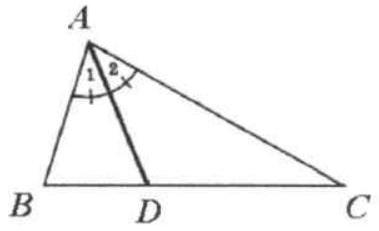
\includegraphics[width=\textwidth]{images/053(1).jpg}

Therefore: \(\frac{A B}{A C}=\frac{B D}{C D}\).

Theorem 3.2. Any point on the bisector of an angle is equidistant from the sides of the angle.\\
\centering
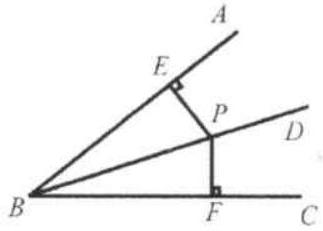
\includegraphics[width=\textwidth]{images/053(2).jpg}

Construct congruent triangles using the angle bisector.
(1). \(B D\) is the angle bisector of \(\angle A B C\). \(P\) is the point on \(B D\). Drawing \(P E \perp A B\), \(P F \perp B C\), we get \(P E=P F . \triangle B P E \cong \triangle B P F\).\\
\centering
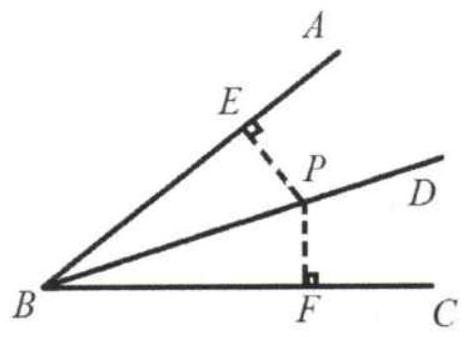
\includegraphics[width=\textwidth]{images/054(1).jpg}\\
(2). \(A B>A C, \angle 1=\angle 2\). Find the point \(E\) on \(A B\) so that \(A E=A C\), and connect \(D E . \triangle A D E \cong \triangle A D C\).\\
\centering
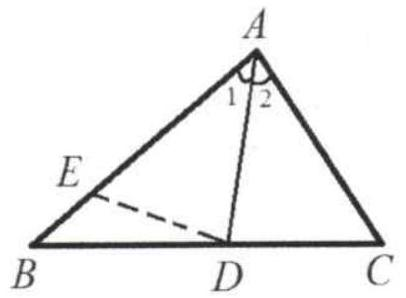
\includegraphics[width=\textwidth]{images/054.jpg}\\
(3). \(\angle 1=\angle 2\). Extend \(A C\) to \(F\) such that \(A F=A B\). Connecting \(D F\), we get \(\triangle A D F\) \(\cong \triangle A D B\).\\
\centering
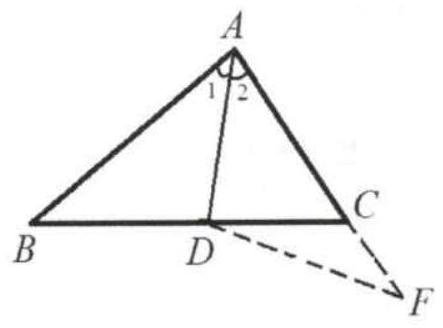
\includegraphics[width=\textwidth]{images/054(2).jpg}

\end{document}
